\chapter{Algorithms} \label{Algorithms}

In this chapter, we will show different algorithms used to obtain the most parsimonious isometric gene tree reconciliation which will be implemented in our software. 

The required input for our algorithms is a rooted species tree with exact branch lengths and an unrooted gene tree with inexact branch lengths. The gene tree is sequentially processed by following algorithms. Firstly, we find all possible roots and root the unrooted tree gene tree, which results in multiple rooted gene trees. Afterwards, we perform the two-pass algorithm (Chapter \ref{two-pass_algorithm}) and count the number of duplications and gene losses for every rooted gene tree to find the most parsimonious reconciliation.

\section{Rooting the gene tree} \label{rooting_the_gene_tree}

We present an algorithm to find possible roots that are distant by given step for every edge $e$ of an unrooted gene tree $G$. 

For each edge $e \in E(G)$, we transform the unrooted gene tree into a semi-rooted gene tree by rooting the subtrees at vertices $u \in V(G)$ and $v \in V(G)$ of the edge $e = (u, v)$. The edge is subsequently used as the parameter for the Algorithm~\ref{getIntervals} to infer intervals for subdividing the given edge and completely root the unrooted gene tree $G$. By default, the $\epsilon$ is set to \num{1e-6} and step to $0.5$.

\begin{algorithm}
\caption{Possible intervals to subdivide given edge $e$} 
\label{getIntervals}
\begin{algorithmic}[1]
\Function{getIntervals}{$e \in E(G), step \in R$}
	\State totalMinLength = $w(e)_{min}$
	\State totalMaxLength = $w(e)_{max}$
	\State minLengthLeft = totalMinLength
	\State maxLengthLeft = totalMaxLength - step
	\State minLengthRight = 0
	\State maxLengthRight = step
	\State difference = totalMaxLength - totalMinLength
	\State differenceIsDivisibleByStep = difference / step == floor(difference / step)
	
	\State intervals.add($\langle 0, \epsilon \rangle$, $\langle totalMinLength, totalMaxLength-\epsilon \rangle$) 
	\State intervals.add($\langle totalMinLength, totalMaxLength-\epsilon \rangle$, $\langle 0, \epsilon \rangle$)
	
	\While {$maxLengthRight < totalMaxLength$ \textbf{and} $maxLengthLeft > 0$ \textbf{and} $step \ne 0$}
		\State intervals.add($\langle minLengthLeft, maxLengthLeft \rangle$, $\langle minLengthRight, maxLengthRight \rangle$)
		\If {$difference = step$ \textbf{or not} $differenceIsDivisibleByStep$}
			\State intervals.add($\langle minLengthRight, maxLengthRight \rangle$, $\langle minLengthhLeft, maxLengthLeft \rangle$)
		\EndIf
		\State minLengthLeft -= step
		\If {$minLengthLeft < 0$}
			\State minLengthLeft = 0
		\EndIf
		\State maxLengthLeft -=step
		\State minLengthRight += step
		\State maxLengthRight += step
	\EndWhile
	\Return {intervals}
\EndFunction
\end{algorithmic}
\end{algorithm}

At the beginning of the Algorithm \ref{getIntervals}, we define essential variables. Possible intervals for subdividing the edge $e$ are stored at the variable \emph{interval} that is also return value of the function. To cover most of the possibilities, we allow rooting the gene tree right above the vertices $u$ and $v$ of the edge $e$. Let $r$ be the root of a semi-rooted gene tree $G$ then we get two possible roots after subdividing the edge $e$ right above the vertices $u$ and $v$. The first possible root subdivide the edge $e$ into two edges with interval lengths $w(u, r) = \langle 0, \epsilon \rangle$ on the left from the root and $w(r, v) = \langle totalMinLength, totalMaxLength-\epsilon \rangle$ on the right from the root, where $w(e)_{min}$ is original minimal length of the edge $e$ and $totalMaxLength$ is original maximal length of the edge $e$. The second option of the root subdivide the edge $e$ with intervals of the same length, that are flipped, so the original interval $w(u, r) = \langle totalMinLength, totalMaxLength-\epsilon \rangle$ is on the left from the root  and $w(r, v) = \langle 0, \epsilon \rangle$ in on the right from the root.

After inferring the first two options of the possible root, we run a while loop to get possible roots inside the edge $e$. In each iteration, we subtract the step from the minimal and maximal length of the left interval of the subdivided edge $e$ and add a step to the minimal and maximal length of the right interval of the subdivided edge $e$. We added condition for special cases, where the difference between the maximal and minimal original length of edge $e$ is equal to step or when it is not divisible by step (Fig. \ref{finding_root}). With the special case condition, we can infer intervals that would be normally skipped. The while loop goes until the maximal length of the right interval is the same or bigger as the original maximal length of the edge $e$ or the maximal length of the left interval reaches $0$ or less.

\begin{figure}[ht!]
	\centering
	\label{finding_root}
  	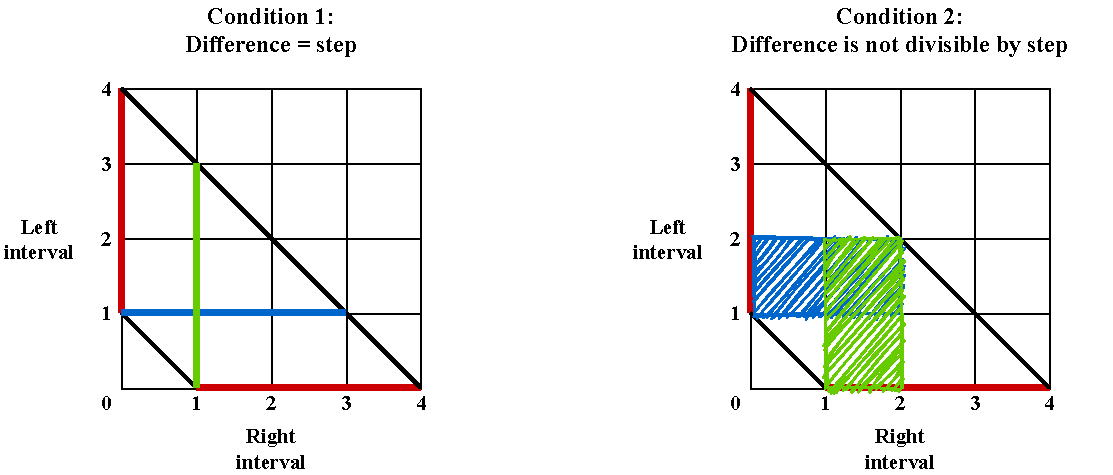
\includegraphics[width=\linewidth]{finding_root}
  	\caption[Rooting the gene tree: special case condition]
  	{The X-axis on the graph stands for the possible length of interval on the left from the root and the y-axis signify the possible length of interval on the right from the root. Space between black lines represents all possible intervals after subdividing the edge $e$ with the root. Red lines are for the root right above the vertices $u$ and $v$, where one interval takes the original size and the second interval is between $0$ and $\epsilon$. Blue lines mean intervals for the root inside the edge $e$ without the special case condition. Green lines are inferred intervals for the root with special case condition \\
  	\textbf{Condition 1}\\
  	Parameters: $w(e) = \langle 1, 4 \rangle$ and $step = 3$. \\
  	In this case, the difference between the original minimal and maximal length is equal to the size of the step. Without the special case condition, we would only get the blue line intervals $w(u, r) = \langle 1, 1 \rangle$ on the left from the root and $w(r, v) = \langle 0, 3 \rangle$ on the right from root. The special case condition flip the intervals thus we get green intervals $w(u, r) = \langle 0, 3 \rangle$ on the left from the root and $w(r, v) = \langle 1, 1 \rangle$ on the right from the root.\\
  	\textbf{Condition 2}\\
  	Parameters: $w(e) = \langle 1, 4 \rangle$ and $step = 2$. \\
  	The difference between original minimal and maximal length is not divisible by the size of step, which give us only the blue lines intervals $w(u, r) = \langle 1, 2 \rangle$ on the left from the root and $w(r, v) = \langle 0, 2 \rangle$ on the right from root without the special case condition. After flipping the intervals with special case condition, we get green intervals $w(u, r) = \langle 0, 2 \rangle$ on the left from the root and $w(r, v) = \langle 1, 2 \rangle$ on the right from the root. Green and blue intervals intersect in area of $\langle 1, 2 \rangle$ for left interval and $\langle 1, 2 \rangle$ for right interval, but it also give us a new area of $\langle 0, 1 \rangle$ for left interval and $\langle 1, 2 \rangle$ for right interval.}
\end{figure}

Rooting the gene tree goes over all edges in the unrooted gene tree $G$. The running time of the function \emph{getIntervals} in Algorithm~\ref{getIntervals} is $O(p)$, where $p$ stands for number of iterations in while loop that can be expressed as $p = ceil(totalMaxLength/step) - 1$. The result of function \emph{getIntervals} is a set of intervals for subdividing the edge $e$. Subsequently, the intervals are used for a loop to root the semi-rooted gene tree $G$ resulting in a set of rooted gene trees with inexact branch lengths, which running time is $O(m)$ for $m = p+2$. Therefore, the total running time of rooting the unrooted gene tree $G$ is $O(Nm)$ with $N$ being the number of all edges in the unrooted tree $G$.


\section{Counting algorithm} \label{counting_algorithm}

We present an algorithm for counting the number of duplications and gene losses in a rooted gene tree $G$ with inexact branch lengths depending on a rooted species tree $S$ with exact branch lengths. We allow only evolutionary events as duplication, gene loss and speciation can happen in evolutionary history. The counting algorithm consists of two parts: preprocessing and the main algorithm. In the preprocessing, we compute essential variables for the gene tree $G$ that are subsequently used in the main algorithm.

The prerequisites for the counting algorithm are calculated depth $D(a)$ and level $l(a)$ for each $a \in V(S)$. For the gene tree $G$, we assume an interval of possible mapping depths $X[u] = \langle X[u]_{min}, X[u]_{max} \rangle$ for each $u \in V(G)$ that can be computed with the two-pass algorithm (Chapter \ref{two-pass_algorithm}) and LCA-mapping $\sigma(u)$ for each $u \in V(G)$.

\subsection{Preprocessing} \label{preprocessing}

In the preprocessing, we calculate necessary variables for nodes in the gene tree $G$ that are used in the main algorithm \ref{main_algorithm}. For each $u \in V(G)$ we compute $l(u)$, $speciesNodeBelow(u)$, $levelDistanceFromParent(u)$ and $mappedToLca(u)$. The level $l(u)$ variable of gene node $u$ signifies number of species nodes on the path from gene node $u$ to the root of the gene tree $G$. It is calculated from the $speciesNodeBelow(u)$ variable that represents species node $s \in V(S)$, which is right below gene node $u$, so the gene node $u$ lies on the path from species node $s$ to $parent(s)$. The $levelDistanceFromParent(u)$ means number of species nodes between gene node $u$ and its $parent(u)$. It is not calculated for the root of the gene tree $G$ as it has no parent. The variable $mappedToLca(u)$ presents the truth value of statement: $X[u]_{max} = D(\sigma(u))$, thus if the node $u$ is mapped to $\sigma(u)$ or not. 

We use three algorithms for calculating the variables: Algorithm~\ref{computeSpeciesNodeBelow} for calculating the $speciesNodeBelow(u)$, Algorithm~\ref{levelDistanceFromChildren} that sets level distance from parent $u \in V(G)$ to its children $\forall v \in children(u): levelDistanceFromParent(v)$ and Algorithm~\ref{computeLevel}, which uses both previous algorithms and computes the level of gene node $l(u)$ and $mappedToLca(u)$.

\begin{algorithm}
\caption{Computes species node below given gene node $u$} 
\label{computeSpeciesNodeBelow}
\begin{algorithmic}[1]
\Function{computeSpeciesNodeBelow}{$u \in V(G), s \in V(S)$} 
	\State speciesNodeBelow = s
	\While {$D(s) > X[u]_{max}$}
		\State speciesNodeBelow = s
		\If {$parent(s) = null$}
			\State \textbf{break}
		\Else
			\State s = parent(s)
		\EndIf
	\EndWhile
	\Return {speciesNodeBelow}
\EndFunction
\end{algorithmic}
\end{algorithm}

The \emph{computeSpeciesNodeBelow} function in Algorithm~\ref{computeSpeciesNodeBelow} saves the given species node $s$ to the variable \emph{speciesNodeBelow}. It always remembers the last species node below the given gene node $u$ and serves as a return value. The while loop iterates over species nodes on the path from given species node $s$ to the root of the species tree. If $D(s) > X[u]_{max}$ stands, it means the species node $s$ is below the gene node $u$. Every iteration, we save the species node to the return value \emph{speciesNodeBelow} and move on the path closer to the root by assigning $parent(s)$ to the $s$ variable. If the species node $s$ does not have a parent, the gene node $u$ is above the root of the species tree. The while loop ends, if the while condition does not stand, so the new species node $s$ is above gene node $u$ or if the gene node $u$ is above the root.

\begin{algorithm}
\caption{Sets level distance from parent to children of node $u$} 
\label{levelDistanceFromChildren}
\begin{algorithmic}[1]
\Function{levelDistanceFromChildren}{$u \in V(G)$} 
	\For {$v \in children(u)$}
		\State levelDistanceFromParent(v) = l(v) - l(u) - mappedToLca(u)
	\EndFor
\EndFunction
\end{algorithmic}
\end{algorithm}

In the \emph{levelDistanceFromChildren} function show in Algorithm~\ref{levelDistanceFromChildren}, we compute the $levelDistanceFromParent(v)$ for each child $v$ of the given node $u$. The level distance is calculated as the difference between the level of child $v$ and the level of its parent, node $u$. The distance is subtracted by 1 if the node $u$ is mapped to the same depth as its $\sigma(u)$.

\begin{algorithm}
\caption{Compute levels for nodes from gene tree $G$} 
\label{computeLevel}
\begin{algorithmic}[1]
\Function{computeLevel}{$u \in V(G)$} 
	\If {$u \in L(G)$}
		\State mappedToLca(u) = true
		\State speciesNodeBelow(u) = $\sigma(u)$
		\State l(u) = l($\sigma(u)$)
	\Else
		\For {$v \in children(u)$}
			\State computeLevel(v)
		\EndFor
		\State depthDifference = $D(\sigma(u)) - X[u]_{max}$
		\If {$X[u]_{max} < D(\sigma(u))$ or $depthDifference > \epsilon$}
			\State mappedToLca(u) = false
			\State node = max($v \in children(u)$: speciesNodeBelow(v))
			\State speciesNodeBelow(u) = computeSpeciesNodeBelow(u, node))
		\Else
			\If {$\forall v \in children(u): speciesNodeBelow(v) = \sigma(u)$}
				\If {$\forall v \in children(u): mappedToLca(v)$}
					\State mappedToLca($v \in children(u): min(v)$) = false
				\EndIf
				\State mappedToLca(u) = false
			\ElsIf {$\exists v \in children(u): speciesNodeBelow(v) = \sigma(u)$}
				\State mappedToLca(u) = false
			\Else
				\State mappedToLca(u) = true
			\EndIf
			\State speciesNodeBelow(u) = $\sigma(u)$
		\EndIf
		\State l(u) = l(speciesNodeBelow(u))
		\State levelDistanceFromChildren(u)
	\EndIf
\EndFunction
\end{algorithmic}
\end{algorithm}

The \emph{computeLevel} function in Algorithm~\ref{computeLevel} goes over all nodes in gene tree $G$ in the direction from the leaves to the root. The leaves of gene tree $t \in L(G)$ are always mapped to its $\sigma(t)$ and their variables are set according to it. For each inner node $u \in V(G) \setminus L(G)$, we recognize whether the node $u$ has the same maximal mapping depth $X[u]_{max}$ as $\sigma(u)$ or the difference between $X[u]_{max}$ and $\sigma(u)$ is smaller than $\epsilon$, which allows us to determine if the node $u$ is mapped to its $\sigma(u)$ even when the depths are not same because of the rounding error. By default, the $\epsilon$ is set to \num{1e-6}.

In case that node $u$ has not the same depth as $\sigma(u)$ and also their \emph{depthDifference} is bigger than $\epsilon$, we set $mappedToLca(u)$ to false. From the children of node $u$, we save the closest species node to the gene node $u$ into variable \emph{node} and run function \emph{computeSpeciesNodeBelow} in Algorithm~\ref{computeSpeciesNodeBelow} to get $speciesNodeBelow(u)$. 

Otherwise, when the node $u$ has the same depth as $\sigma(u)$ or the \emph{depthDifference} is smaller or equal to the $\epsilon$, we consider three cases can happen, where the first two cases check if both or at least one child is already mapped to $\sigma(u)$, because exactly one node from the gene tree can be mapped to exactly one node from species tree to be considerate as speciation. In the first case, we consider that both $v \in children(u)$ have the same $speciesNodeBelow(v)$ as $\sigma(u)$. It means that both children of node $u$ can be mapped to the same species node, so we check if their $mappedToLca(v)$ is set to true. If the condition holds, we take the child $v$ that is closer to the node $u$ and set its $mappedToLca(v)$ to false. As the other child is already mapped to the species node, we set $mappedToLca(u)$ to false.

The second case checks if at least one $v \in children(u)$ is mapped to $\sigma(u)$. If the condition holds, we can not map another gene node to the species node, so we set $mappedToLca(u)$ to false. 

In the third case, any $v \in children (u)$ has the same $speciesNodeBelow(v)$ as the $\sigma(u)$, thus we set the $mappedToLca$ to true.

Lastly, we set the $speciesNodeBelow(u)$ to the $\sigma(u)$ and level of node $u$ to the level of computed $speciesNodeBelow(u)$. Then, we run function \emph{levelDistanceFromChildre} in Algorithm~\ref{levelDistanceFromChildren}.

The \emph{computeLevel} function goes over all nodes in the rooted gene tree $G$. If the gene tree $G$ is balanced, the function \emph{computeSpeciesNodeBelow} has running time $O(log N)$, where $N$ is number of nodes in gene tree $G$. The \emph{levelDistanceFromChildren} function is computed in constant time. So the total preprocessing running time is $O(N log N)$ for balanced gene tree $G$. However, if the gene tree $G$ is not balanced, the preprocessing running time is $O(N^2)$.

\subsection{Main algorithm} \label{main_algorithm}

The prerequisites for the \emph{countDL} function shown in Algorithm~\ref{countDL} are computed in preprocessing. Besides, we need to have set the \emph{countLossesAboveRoot} variable. If it is true, we count losses above root that occurred as a result of the gene tree $G$ not containing genes of all species from the species tree $S$. 

\begin{algorithm}
\caption{Counts duplications and gene losses in gene tree $G$} 
\label{countDL}
\begin{algorithmic}[1]
\Function{countDL}{$u \in V(G)$} 
	\If {$u \ne L(G)$}
		\State v, w = children(u)
		\State $DL_u = DL_v+DL_w$
	\EndIf

	\State loss = levelDistanceFromParent(u)
	\If {$parent(u) = null$ \textbf{and} $parent(\sigma(u)) \ne null$ \textbf{and} $countLossesAboveRoot$}
		\State loss += l(u); 
	\EndIf
	\If {\textbf{not} $mappedToLca(u)$}
		\State duplication = 1
	\EndIf
	
	\Return {$DL_u$ +(duplication, loss)}
\EndFunction
\end{algorithmic}
\end{algorithm}

We count the evolutionary events in the direction from leaves to the root of gene tree $G$. For each node $u \in V(G)$ and its parent $v \in V(G)$, we consider evolutionary events that occur in the node $u$ and on the edge $(u, v)$. We do not compute evolutionary event in the parent, they are determined directly in the parent. In the root, we only calculate the evolutionary events that happened in the node as the root has no parent thus no edge to consider.

The number of duplications and gene losses are depicted as pair $DL = (duplication, loss)$. The sum of the pairs $DL_1$  and $DL_2$ is computed as $DL_1+DL_2=(duplication_1+duplication_2, loss_1+loss_2)$. For each node $u \in V(G)$, we calculate the $DL_u$, which corresponds to the number of duplications and gene losses inferred in the subtree of node $u$. Thereafter, we infer the duplication and gene losses in the node $u$ and on the edge above the node $u$.

The number of gene losses on the edge $(u, v)$ is calculated as the number of species nodes on the path from node $u$ to node $v$, which is precomputed in variable $levelDistanceFromParent(u)$. If $\sigma(root(G)) \ne root(S)$, thus the $\sigma(root(G))$ is below $root(S)$ means that some species do not have their gene in the gene tree. Therefore, the gene loss occurred before the $root(G)$, which resolves in extra gene loss that can be added if the variable \emph{countLossesAboveRoot} is true. The truth value of \emph{countLossesAboveRoot} is set by the user.

Duplication and speciation are easy to determine since it depends on whether the node $u$ is mapped to $\sigma(u)$ or above, which we already precomputed in $mappedToLca(u)$.

The function return pair $DL$ corresponds to the number of duplication and gene losses in the subtree of node $u$, in the node $u$ and on the edge above node $u$.

Gene losses and duplications are computed in constant time for one gene node. The \emph{countDL} function goes over all nodes in gene tree $G$ thus the running time is $O(N)$, where $N$ is the number of all node in the gene tree $G$.


